\documentclass[11pt,a4paper]{article}
\usepackage[utf8x]{inputenc}
\usepackage{graphicx}
\usepackage{esdiff}
\usepackage[english]{babel}
\usepackage{color}
\usepackage{float}
\usepackage{enumitem}
\usepackage{epstopdf}
\usepackage{afterpage}
\usepackage{caption}
\usepackage{subcaption}
\captionsetup[table]{oneside , margin = {2cm, 0cm},
	justification=RaggedRight, singlelinecheck = false }
\usepackage{subcaption}
\usepackage{mathtools}
\usepackage{multicol}
\usepackage{algorithm2e}
\usepackage{microtype}
\usepackage{titling}
\usepackage{amsmath}
\usepackage{verbatim}
\usepackage[colorlinks=true]{hyperref} % the option is there to remove the square around links which is what I don't like.
\usepackage{comment}
\usepackage{perpage} 
\MakePerPage{footnote} % Reset the footnote counter perpage. may require to run latex twice.
\usepackage{commath} % for absolute value
\usepackage[margin=2cm]{geometry} % This is here to fit more text into the page.

\setcounter{secnumdepth}{1}  % This removes the numbering from the subsections.
% If you want the numbering of the subsection level just remove this line
\usepackage{titling}
\newcommand{\subtitle}[1]{%
	\posttitle{%
		\par\end{center}
	\begin{center}\large#1\end{center}
	\vskip0.5em}%
}

\setlength{\parindent}{0pt} % No indentation for paragraphs. Because that is just old.
\setlength{\parskip}{\baselineskip} % Instead use vertical paragraph spacing.

\fontencoding{T1} % the better font encoding.
\title{\textsc{Final project \\ \bigskip Design of an active suspension system}}
\subtitle{\textsc{Automatic Control}}	
%\date{11/06/2020}
\author{Giorgio Checola}

\makeatletter
\def\@maketitle{
\graphicspath{ {./images/} }

\includegraphics[width=100mm]{unitn-logo}
\begin{center}
	
	\item {\Huge \bfseries \@title } 
	
	\bigskip
	
	\item { \Large Automatic Control}
	
	\bigskip
	
	\item {\Large  \@author}  
	
	\bigskip
	
	%\item \@date 
	
	\item matr. 215475
	
	\bigskip
	
	\item Department of Industrial Engineering
	
	\bigskip
	
	\item {Università degli studi di Trento}
	\\
	
\end{center}
}
\makeatother

\begin{document}

\graphicspath{ {./images/} }
\maketitle
\thispagestyle{empty}
%\newpage
\thispagestyle{empty}
\mbox{}
\newpage


\section{Introduction}	
The project concerns a wheel-suspension assembly of a car. When there is no control action on the system the suspension is called "passive", while it is "active" when there is a force, provided by an actuator placed between the wheel center and the car body, that acts as the control input for the system.
My objective has been to solve a simplified version of the problem in order to reduce the impact of an uneven road on the vertical acceleration of the car body.

\section{Answers}
\begin{enumerate}
	\item By considering the passive suspension system (i.e. $u=0$), we can verify if the system is stable with the eigenvalues test: all eigenvalues of the matrix A have negative real part ($Re(\lambda_i) < 0$), so it is stable.
	
	\smallskip
	 
	The convergence rate $\alpha$ is smaller than 1.5 because the biggest eigenvalue of the matrix A is -1.327. It must be verified the inequality $Re(\lambda_i(A)) < -\alpha$.
	
	\smallskip
	
	The $\mathcal{L}_2$ gain of a system is the maximum value of the ratio between  energy of the output and energy of the noise. I can compute this value using the function \texttt{getPeakGain}. The result is: $\mathcal{L}_2=21.4026878512419$. \\
	In the image below we can see the Bode plot of the transfer function of the passive suspension system. The red horizontal line is the value of the $\mathcal{L}_2$ gain obtained before, and it corresponds exactly to the peak of the transfer function. 
	
	\smallskip
	
	\begin{figure}[H]
		\centering
		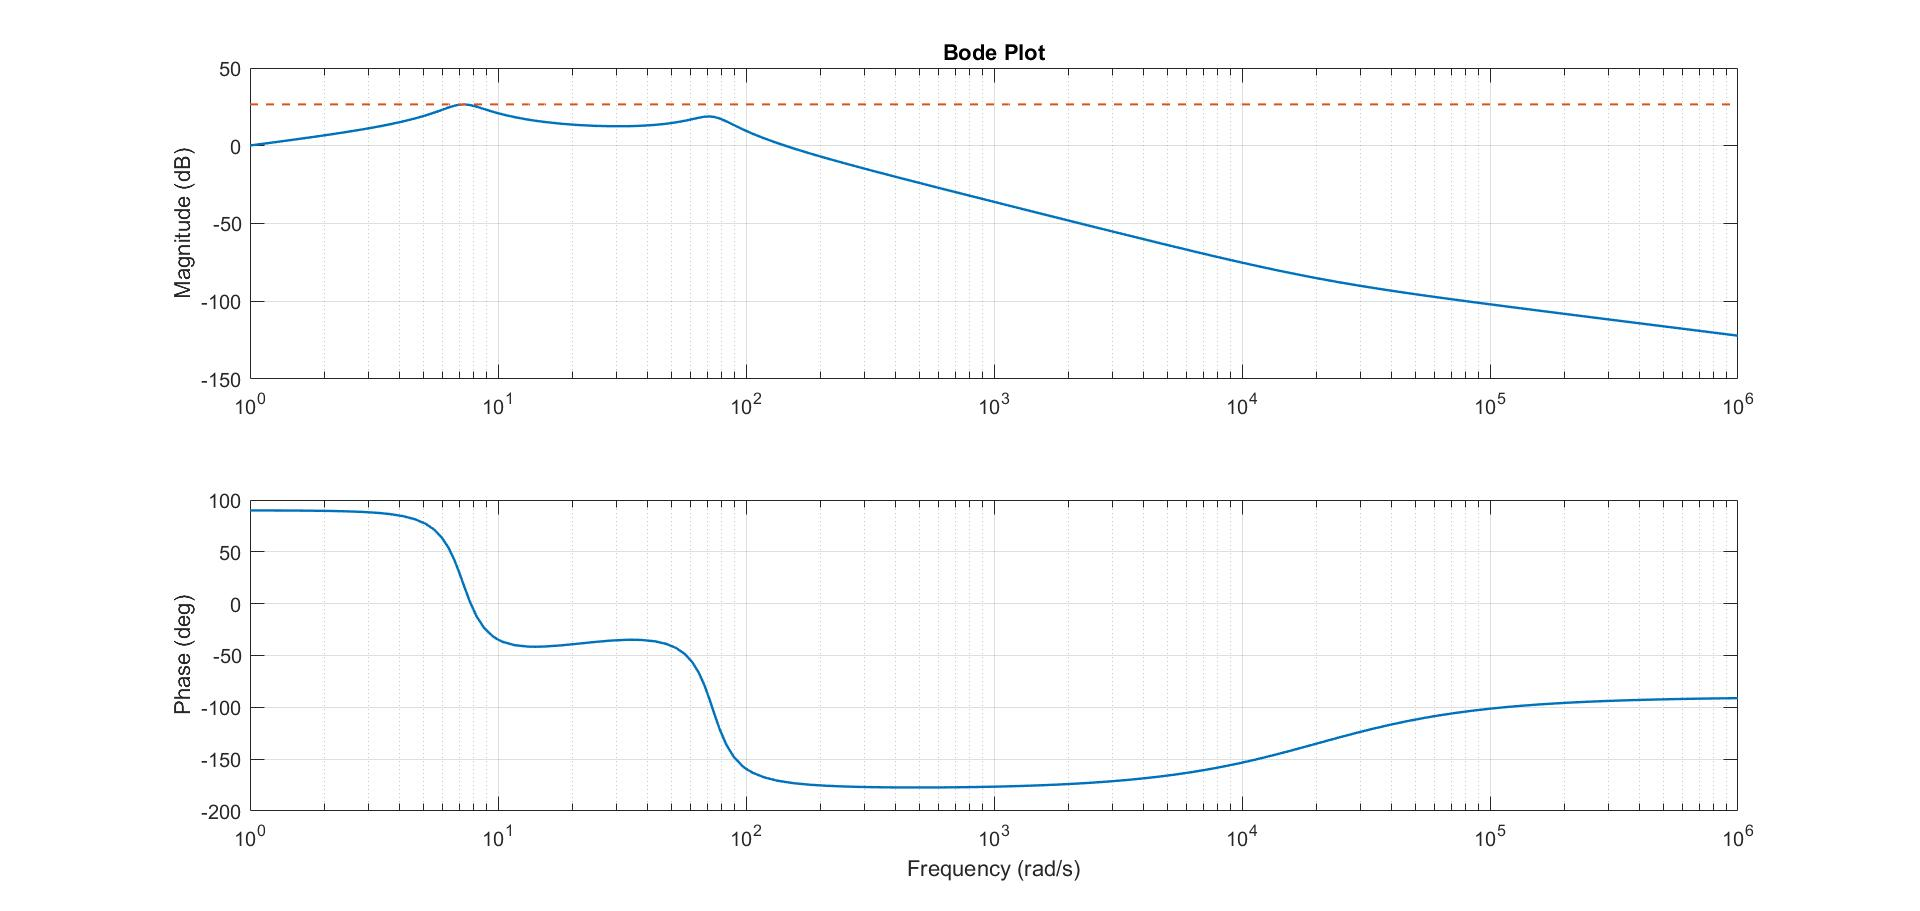
\includegraphics[width=150mm]{plots/gamma_peak.jpg}
		\caption{Bode plot of the open loop system}
		\label{fig:1}
	\end{figure}
	
	\medskip
	
	\item Before synthesizing a full-state feedback controller $u=Kx$ for the active suspension system, we have to know if we can control it, so we check the controllability of the system. \\
	Since the controllability matrix is full rank I can place the real parts of the eigenvalues of the closed-loop system wherever I want in the negative half plane. \\ 
	The constraints of the LMI problem are:
	\begin{equation}
	\begin{cases}
	W \ge \rho I_{nxn} \\ \rho \ge 0 \\
	\begin{bmatrix}
	He(AW+BX) & E & (CW+DX)\textsuperscript{T} \\
	E\textsuperscript{T} &   -\gamma \cdot I_{dxd}  & F\textsuperscript{T}  \\
	(CW+DX) & F & -\gamma \cdot I_{mxm}
	\end{bmatrix} \leq 0\\
	
	\begin{bmatrix}
	k \cdot \rho \cdot I_{nxn} &      X\textsuperscript{T} \\
	X &        k\cdot \rho \cdot I_{pxp} 
	\end{bmatrix} \ge 0
	\end{cases}  
	\end{equation}
	The matrix $K$ needs to have norm $k$ smaller than $2\cdot10^5$, so I fix this value and I search for the desired controller and its parameters: by means of the solver I find the optimal solution for $\gamma$, and then $K$ with the corresponding matrix $M$ and $X$.
	
	\begin{itemize}
		\item[$\rightarrow$] $K_a= \begin{bmatrix} 12879.7774 & 30131.0741 & -52.2964489 & 94.2500777 \end{bmatrix}$
		\item[$\rightarrow$] $\alpha_a=1.3828$
		\item[$\rightarrow$] $\gamma_a=9.2275$
		
	\end{itemize}	

	As you can see, we confirm that it is possible to obtain a $\mathcal{L}_2$ smaller than 10. The following picture shows the Bode plot of the closed loop system.
	
	\medskip
	
	\begin{figure}[H]
		\centering
		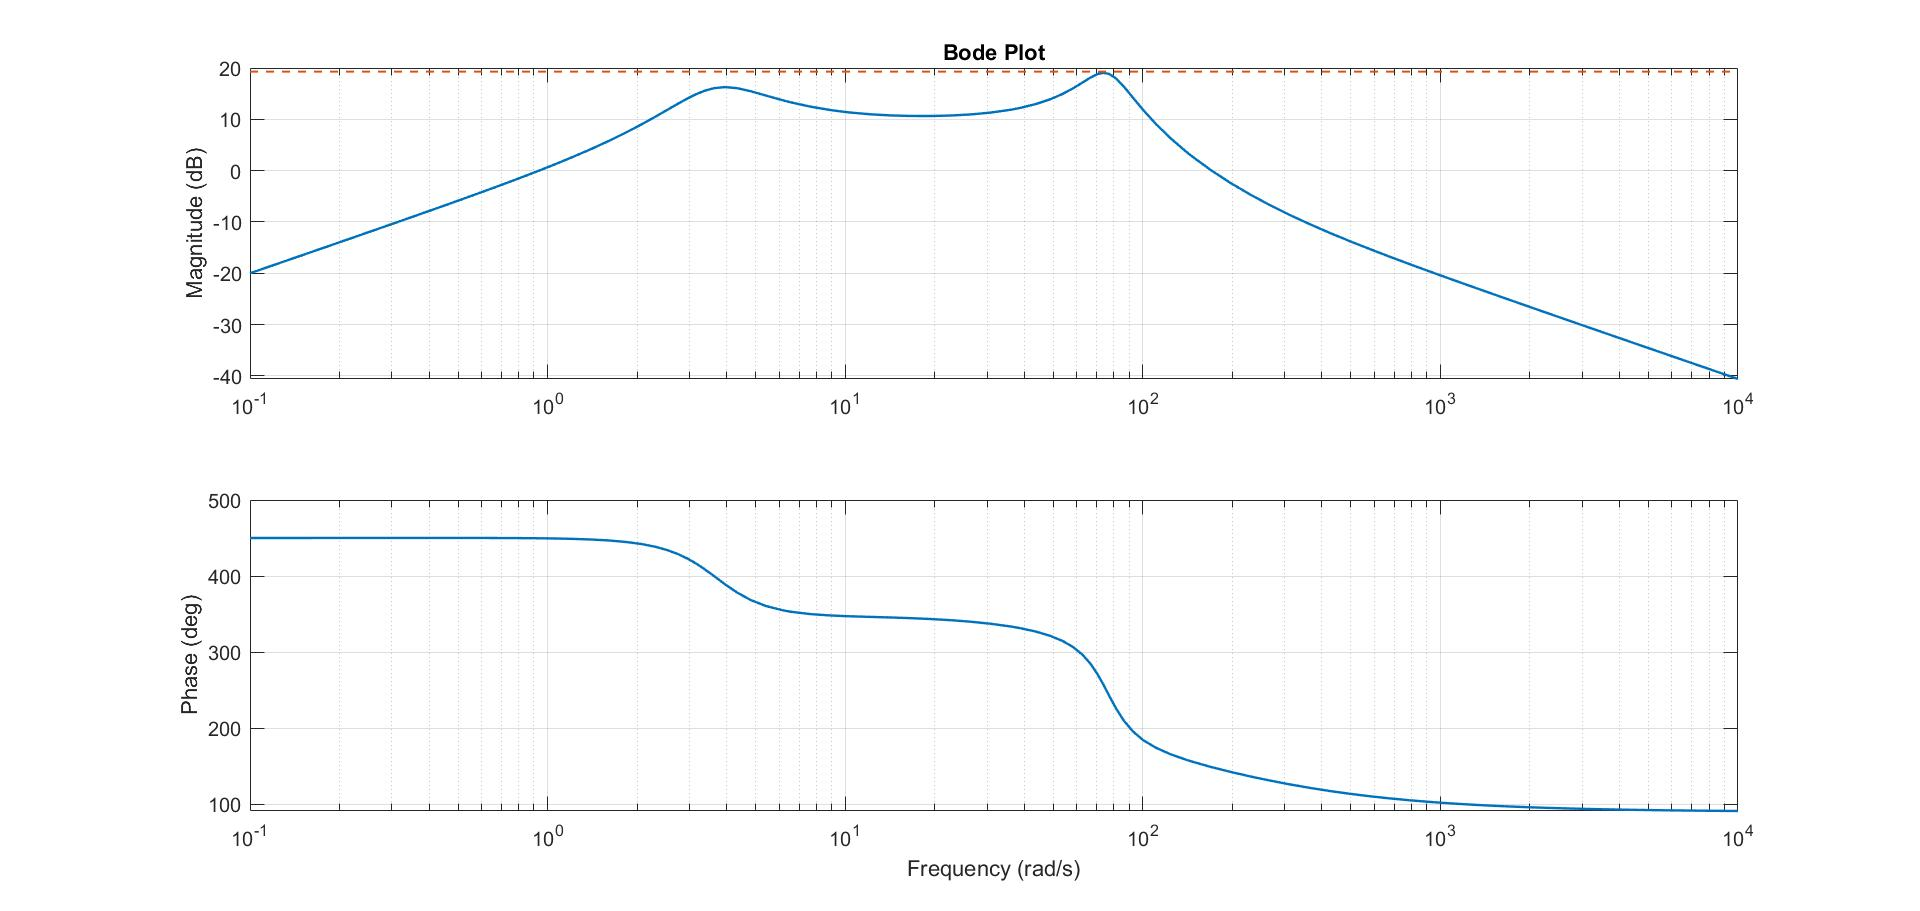
\includegraphics[width=150mm]{plots/gamma_a.jpg}
		\caption{Bode plot of the closed loop system ($k=2\cdot10^5$)}
		\label{fig:2}
	\end{figure}
	
	\item In order to obtain a convergence rate $\alpha$ greater than 1.5, I have to find a new matrix $K$ such that $Re(\lambda_i(A_{cl})) < -1.5$. I can get it by solving the previous LMI (I keep the norm value $k$ fixed) with an additional constraint: He$(AW+BX)\leq-2\alpha^\ast W$ where $\alpha^\ast=1.5$. 
	
	
	Finally I obtain these results:
	\begin{itemize}
		\item[$\rightarrow$] $K_b= \begin{bmatrix} 11691.6768 & 37832.7639 & -875.028917 & 78.4479637 \end{bmatrix}$
		\item[$\rightarrow$] $\alpha_b=2.4143$
		\item[$\rightarrow$] $\gamma_b=10.3393$
	\end{itemize}
	The new matrix $A_{cl}$ has all the eigenvalues with real part smaller than $-\alpha_b$. \\
	The Bode plot of the new transfer function of the system is shown below.
	
	\begin{figure}[H]
		\centering
		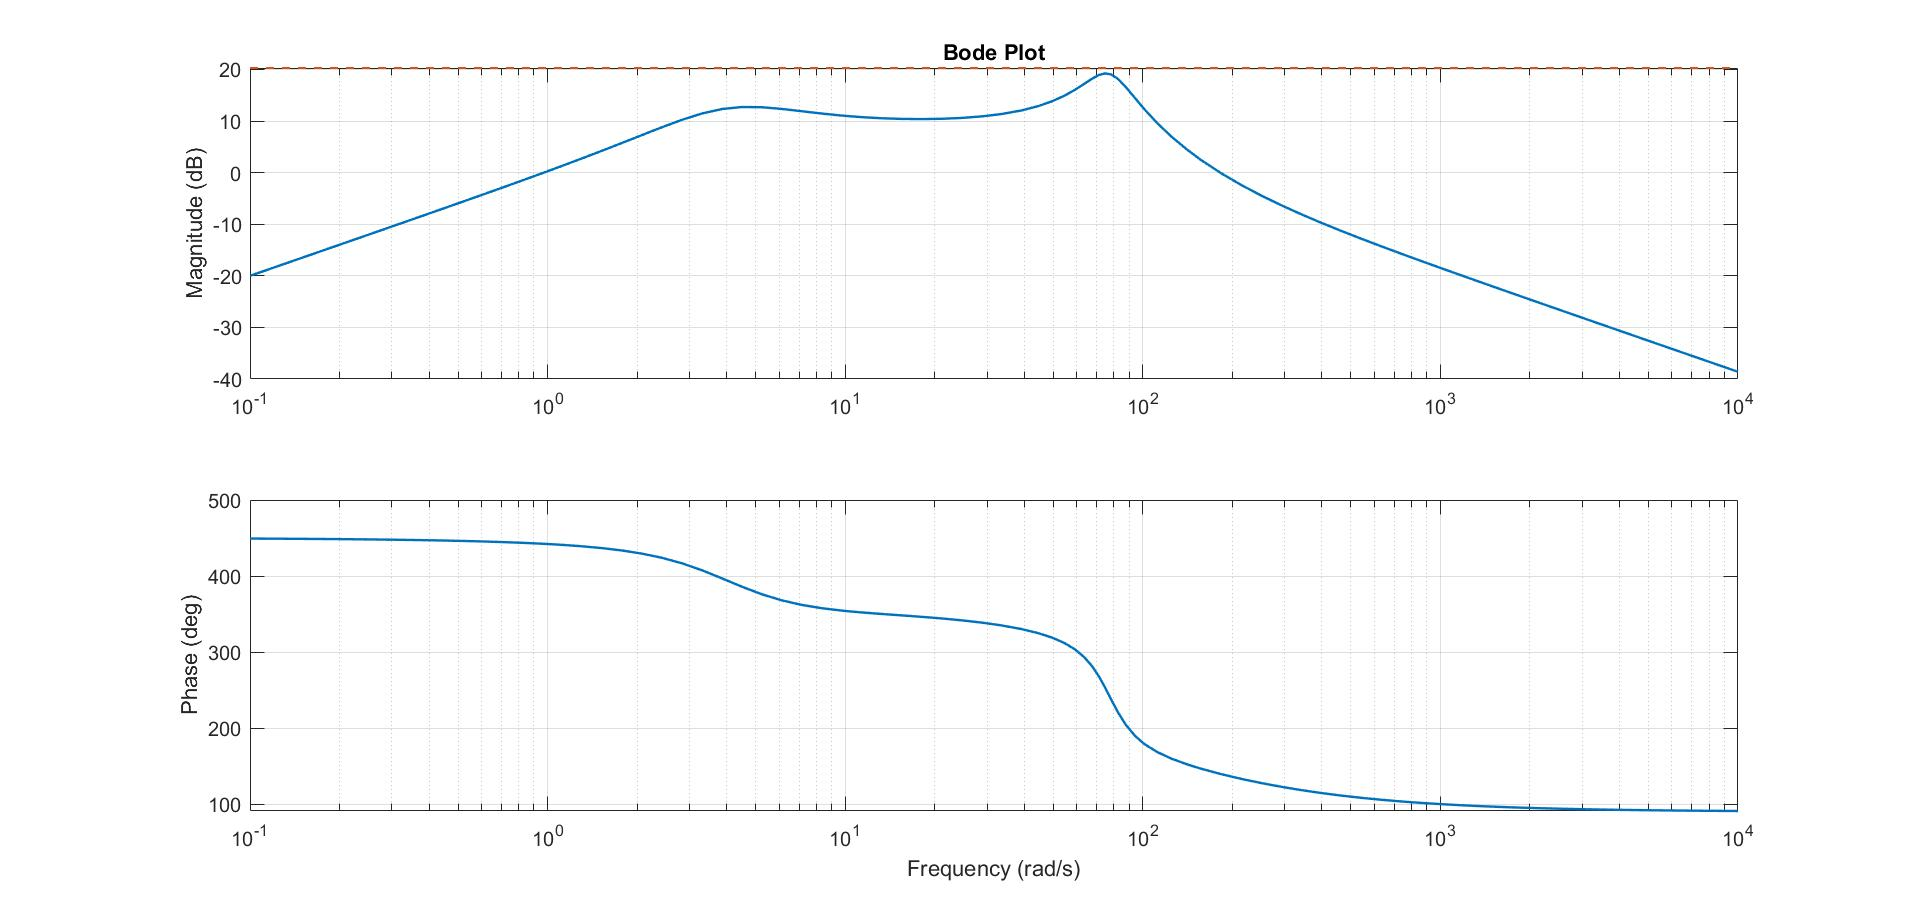
\includegraphics[width=150mm]{plots/gamma_b.jpg}
		\caption{Bode plot of the closed loop system ($k=2\cdot10^5$ and $\alpha>1.5$)}
		\label{fig:3}
	\end{figure}
	 Despite the results of the two cases I think it is possible to obtain a controller which satisfies both requirements ($\gamma<10$ and $\alpha>1.5$).
	
	\item If you use an optimization solver with both requirements as input, you get the following gain matrix $K$:
	\begin{equation}
		K_c= \begin{bmatrix} 12674 & 31347 & -168.3 & 92.5 \end{bmatrix}
	\end{equation}
	and the corresponding $\mathcal{L}_2$ gain and convergence rate $\alpha$ that satisfy the conditions ($\gamma_c=9.35$ and $\alpha_c=1.53$).\\ With my LMI formulation I didn't obtain this result because I am looking for a single Lyapunov function that satisfies two different conditions, but it is wrong. I should use two functions with different matrix variables, but then the problem would become nonconvex, and I can't solve it with LMI anymore.
	
\end{enumerate}
\newpage
\hypersetup{linkcolor = black}
\listoffigures
\end{document}

